% Syllabus Template from Arman Shokrollahi
% https://www.overleaf.com/latex/templates/syllabus-template-course-info/gbqbpcdgvxjs

\documentclass[11pt, letterpaper]{article}
%\usepackage{geometry}
\usepackage[inner=2cm,outer=2cm,top=2.5cm,bottom=2.5cm]{geometry}
\pagestyle{empty}
\usepackage{graphicx}
\usepackage{fancyhdr, lastpage, bbding, pmboxdraw}
\usepackage[usenames,dvipsnames]{color}
\definecolor{darkblue}{rgb}{0,0,.6}
\definecolor{darkred}{rgb}{.7,0,0}
\definecolor{darkgreen}{rgb}{0,.6,0}
\definecolor{red}{rgb}{.98,0,0}
\usepackage[colorlinks,pagebackref,pdfusetitle,urlcolor=darkblue,citecolor=darkblue,linkcolor=darkred,bookmarksnumbered,plainpages=false]{hyperref}
\renewcommand{\thefootnote}{\fnsymbol{footnote}}

\pagestyle{fancyplain}
\fancyhf{}
\lhead{ \fancyplain{}{Text As Data} }
%\chead{ \fancyplain{}{} }
\rhead{ \fancyplain{}{Maymester 2022} }%\today
%\rfoot{\fancyplain{}{page \thepage\ of \pageref{LastPage}}}
\fancyfoot[RO, LE] {page \thepage\ of \pageref{LastPage} }
\thispagestyle{plain}

%%%%%%%%%%%% LISTING %%%
\usepackage{listings}
\usepackage{caption}
\DeclareCaptionFont{white}{\color{white}}
\DeclareCaptionFormat{listing}{\colorbox{gray}{\parbox{\textwidth}{#1#2#3}}}
\captionsetup[lstlisting]{format=listing,labelfont=white,textfont=white}
\usepackage{verbatim} % used to display code
\usepackage{fancyvrb}
\usepackage{acronym}
\usepackage{amsthm}
\VerbatimFootnotes % Required, otherwise verbatim does not work in footnotes!



\definecolor{OliveGreen}{cmyk}{0.64,0,0.95,0.40}
\definecolor{CadetBlue}{cmyk}{0.62,0.57,0.23,0}
\definecolor{lightlightgray}{gray}{0.93}



\lstset{
%language=bash,                          % Code langugage
basicstyle=\ttfamily,                   % Code font, Examples: \footnotesize, \ttfamily
keywordstyle=\color{OliveGreen},        % Keywords font ('*' = uppercase)
commentstyle=\color{gray},              % Comments font
numbers=left,                           % Line nums position
numberstyle=\tiny,                      % Line-numbers fonts
stepnumber=1,                           % Step between two line-numbers
numbersep=5pt,                          % How far are line-numbers from code
backgroundcolor=\color{lightlightgray}, % Choose background color
frame=none,                             % A frame around the code
tabsize=2,                              % Default tab size
captionpos=t,                           % Caption-position = bottom
breaklines=true,                        % Automatic line breaking?
breakatwhitespace=false,                % Automatic breaks only at whitespace?
showspaces=false,                       % Dont make spaces visible
showtabs=false,                         % Dont make tabls visible
columns=flexible,                       % Column format
morekeywords={__global__, __device__},  % CUDA specific keywords
}

%%%%%%%%%%%%%%%%%%%%%%%%%%%%%%%%%%%%
\begin{document}
\begin{center}
{\Large \textsc{POLS 8500: Text As Data}}
\end{center}
\begin{center}
{\large Maymester 2022}
\end{center}

\begin{center}
\rule{6.5in}{0.4pt}
\begin{minipage}[t]{.96\textwidth}
\begin{tabular}{llcccll}
\textbf{Professor:} & Joe Ornstein & & &  & \textbf{Time:} & MTWThF 11:00am -- 1:45pm \\
\textbf{Email:} &  \href{mailto:jornstein@uga.edu}{jornstein@uga.edu} & & & & \textbf{Place:} & 101D Baldwin Hall\\
\textbf{Website:} & \href{https://github.com/joeornstein/maymester-text-as-data-2022}{maymester-text-as-data-2022} & & & & &
\end{tabular}
\end{minipage}
\rule{6.5in}{0.4pt}
\end{center}
\vspace{.15cm}
\setlength{\unitlength}{1in}
\renewcommand{\arraystretch}{2}


\noindent So much information about our political world is stored not in tidy datasets, but in \textit{texts}. Party manifestos, social media posts, city council minutes, email correspondence, treaties, ordinances, judicial decisions, presidential debates, Congressional speeches....the practice of politics in its myriad forms ultimately comes to be recorded in words on a page. How do we take all this unstructured text, far too extensive for any one researcher to read, and convert it into useful information for scientific inquiry?

In this class we will explore the cutting edge of ``text-as-data'', with a focus on how to retrieve, represent, and analyze political texts as part of a research project. We will aim to cover both the conceptual and the practical, spending class time writing code to replicate and extend significant results from the past decade of political science research. 

%\begin{figure}[h]
%	\centering
%	\href{https://xkcd.com/1856/}{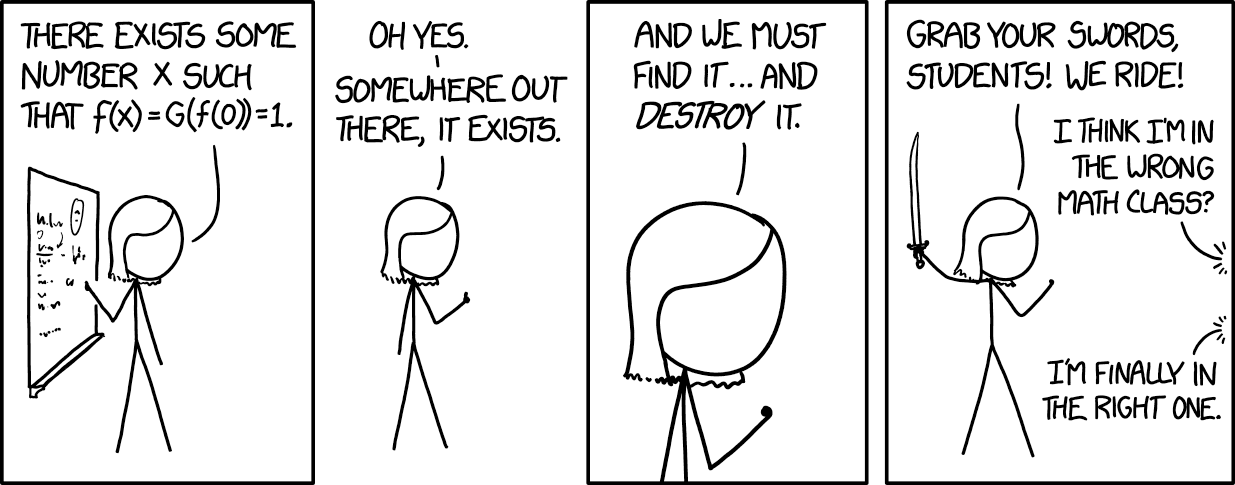
\includegraphics[width=0.8\textwidth]{img/existence_proof_2x.png}}
%\end{figure}

%\begin{quotation}
%	\noindent``\textit{You can't really know anything if you just remember isolated facts. If the facts don't hang together on a latticework of theory, you don't have them in a usable form. You've got to have models in your head.}''\\
%	\\
%	--Charlie Munger (investor, vice chairman of Berkshire Hathaway)
%\end{quotation}


\section*{Course Prerequisites and Objectives}
%\vskip.15in
%\noindent\textbf{Course Objectives:}  
I will assume that before taking this course you have taken POLS 7012 and 7014 or their equivalents (introduction to statistics and linear regression) and that you are familiar with the basics of the \texttt{R} programming language. By the end of this course, you will be able to:
\begin{itemize}
	\item Retrieve and clean text data from a variety of sources
	\item Thoughtfully measure and quantify concepts of interest to your research using text data
	\item Fit machine learning models for clustering, sentiment analysis, topic classification, and prediction
\end{itemize}


\section*{Assignments \& Grading}

There will be daily coding activities in class designed to apply the concepts we learn to practical research problems. Your grade will be based on the successful completion of these assignments. 

%\vskip.15in
%\noindent\textbf{Office Hours:} 
\section*{Office Hours}

Since we're meeting for 3 hours every day, I will not hold formal office hours, but I will generally be available before and after class to discuss questions and will respond to emails from 9am to 4pm.

%\vskip.15in
%\noindent\textbf{Textbook:} %\footnotemark
\section*{Textbooks}

For our tour through the world of text as data, we will rely on two textbooks. The first is a a broad conceptual overview of the field of text as data, and the second is a practical introduction to the \texttt{R} code you can use to work with text (and is available online for free at the link below).

\begin{itemize}
\item Grimmer, Justin, Brandon M. Stewart, and Margaret E. Roberts. \textit{Text As Data: A New Framework for Machine Learning and the Social Sciences.} Princeton University Press, 2022.
\item \href{https://www.tidytextmining.com/index.html}{Silge, Julia, and David Robinson. \textit{Text Mining with R: A Tidy Approach.} First edition. O’Reilly, 2017.}
\end{itemize} 



\section*{Tentative Course Outline and Readings}

Please read and markup these readings before class each day.

\subsection*{Day 1: Getting Started}

\textit{What Are We Doing Here? A review of R and RStudio.}

\begin{itemize}
	\item GSR Chapters 1-2
	\item \href{https://joeornstein.github.io/pols-3230/week-11.html#getting-twitter-data}{Instructions to sign up for the Twitter API}
\end{itemize}

\subsection*{Day 2: Creating a Corpus}

\textit{Where and how do we get text data? Playtime with Twitter.}

\begin{itemize}
	\item GSR Chapters 3-4
	\item \href{https://www.tidytextmining.com/tidytext.html}{SR Chapter 1: Tidy Text Data}
\end{itemize}

\subsection*{Day 3: The Bag of Words}

\textit{What if we ignored everything we know about language and just counted the words? Would that get us anywhere?}

\begin{itemize}
	\item GSR Chapter 5
	\item \href{https://www.tidytextmining.com/dtm.html}{SR Chapter 5: Document-Term Matrices}
\end{itemize}

\subsection*{Day 4: Modeling The Bag of Words}

\textit{Probabilistic vs. Algorithmic Models, The Federalist Papers}

\begin{itemize}
	\item GSR Chapters 6-7
\end{itemize}

\subsection*{Day 5: Word Embeddings}

\textit{What if words were actually just a bunch of numbers?}

\begin{itemize}
	\item GSR Chapter 8
	\item Rodriguez, Pedro L., and Arthur Spirling. 2021. ``Word Embeddings: What Works, What Doesn’t, and How to Tell the Difference for Applied Research'' \textit{The Journal of Politics}.
\end{itemize}


\subsection*{Day 6: Text Reuse}

\textit{Let's take a model developed to detect plagiarism and use it to see how ideas spread in political texts over time.}

\begin{itemize}
	\item GSR Chapter 9.1
	\item Wilkerson, John, David Smith, and Nicholas Stramp. 2015. ``Tracing the Flow of Policy Ideas in Legislatures: A Text Reuse Approach.'' \textit{American Journal of Political Science} 59(4): 943–56.
	\item Jansa, Joshua M., Eric R. Hansen, and Virginia H. Gray. 2019. ``Copy and Paste Lawmaking: Legislative Professionalism and Policy Reinvention in the States.'' \textit{American Politics Research} 47(4): 739–67.
\end{itemize}


\subsection*{Day 7: Clustering}

\textit{What if we don't know in advance how we want to measure our concept? Can we just let the computer tell us how to categorize our text data?}

\begin{itemize}
	\item GSR Chapter 10 (Discovery)
	\item GSR Chapter 12 (Clustering)
\end{itemize}



\subsection*{Day 8: Topic Models}

\textit{Latent Dirichlet Allocation (LDA): Not Quite As Frightening As That Name Makes It Seem}

\begin{itemize}
	\item GSR Chapter 13
	\item \href{https://www.tidytextmining.com/topicmodeling.html}{SR Chapter 6}
\end{itemize}

\subsection*{Day 9: Measurement}

\textit{How do you know if you've done a good job measuring something?}

\begin{itemize}
	\item GSR Chapter 15
\end{itemize}


\subsection*{Day 10: Word Counting}

\textit{Dictionary methods and sentiment analysis. What if we just counted up the different kinds of words in a document? Would that be a good measure?}

\begin{itemize}
	\item GSR Chapter 16
	\item \href{https://www.tidytextmining.com/sentiment.html}{SR Chapter 2}
\end{itemize}

\subsection*{Day 11: Supervised Learning, Part 1}

\textit{Step 1: Measure a bunch of documents by hand. Step 2: Get tired of doing it all by hand. Step 3: Ask the computer to predict how it would measure the rest of the documents if it were you. Step 4: Profit.}

\begin{itemize}
	\item GSR Chapter 17
\end{itemize}



\subsection*{Day 12: Crowd-Coding}

\textit{What if we let other people do the hand-coding? MTurk, SentimentIt}

\begin{itemize}
	\item GSR Chapter 18
	\item Carlson, David, and Jacob M. Montgomery (2017). ``A Pairwise Comparison Framework for Fast, Flexible, and Reliable Human Coding of Political Texts.'' \textit{American Political Science Review} 111, no. 4: 835–43.
	
\end{itemize}

\subsection*{Day 13: Supervised Learning, Part 2}

\textit{Naive Bayes, Regularization, Ensembles}

\begin{itemize}
	\item GSR Chapter 19
\end{itemize}

\subsection*{Day 14: Foundation Models}

\textit{Here we bring it all together. Take a massive semi-supervised neural network, train it on the entire Internet, and see what happens.}

\begin{itemize}
	\item GSR Section 8.5
	\item Ornstein, Blasingame, and Truscott (2022). ``How To Train Your Stochastic Parrot.'' \textit{Working Paper}.
	\item Alexander, Scott. 2019. \href{https://slatestarcodex.com/2019/02/19/gpt-2-as-step-toward-general-intelligence/}{``GPT-2 As Step Toward General Intelligence.''} \textit{Slate Star Codex}.
	\item Alexander, Scott. 2020. \href{https://slatestarcodex.com/2020/06/10/the-obligatory-gpt-3-post/}{``The Obligatory GPT-3 Post.''} \textit{Slate Star Codex.}
		
\end{itemize}

\subsection*{Day 15: Bonus Day}

\textit{Catch-up and Topics By Popular Demand}

%\section*{Academic Honesty}
%
%Remember that when you joined the University of Georgia community, you agreed to abide by a code of conduct outlined in the academic honesty policy called \href{https://honesty.uga.edu/Academic-Honesty-Policy/Introduction/}{\textit{A Culture of Honesty}}. 

\section*{Mental Health and Wellness Resources}

\begin{itemize}
\item If you or someone you know needs assistance, you are encouraged to contact Student Care and Outreach in the Division of Student Affairs at 706-542-7774 or visit \href{https://sco.uga.edu}{https://sco.uga.edu}. They will help you navigate any difficult circumstances you may be facing by connecting you with the appropriate resources or services. 
\item UGA has several resources for a student seeking \href{https://www.uhs.uga.edu/bewelluga/bewelluga}{mental health services} or \href{https://www.uhs.uga.edu/info/emergencies}{crisis support}. 
\item If you need help managing stress anxiety, relationships, etc., please visit \href{https://www.uhs.uga.edu/bewelluga/bewelluga}{BeWellUGA} for a list of FREE workshops, classes, mentoring, and health coaching led by licensed clinicians and health educators in the University Health Center.
\item Additional resources can be accessed through the UGA App.
\end{itemize}



%%%%%% THE END 
\end{document} 